\documentclass[../main.tex]{subfiles}

\begin{document}
LSTM (Long Short-Term Memory) là một mạng nơ-ron được sửa đổi dựa trên mạng nơ-ron hồi quy đã nêu ở phần trước cũng với vai trò nắm bắt thông tin phụ thuộc vào các thông tin trước đó. LSTM có khả giải quyết vấn đề phụ thuộc xa bằng cách thêm các cổng cho các ô. Mỗi ô có $2$ trạng thái là mở và đóng, cho phép LSTM có thể hoạt động như bộ nhớ máy tính khi đưa ra quyết định dữ liệu nào được phép ghi  vào, dữ liệu nào được phép đọc và lưu trữ lại. Thêm nữa, LSTM có $4$ mạng nơ-ron tương tác với nhau. 

\begin{figure}[h]
\centering
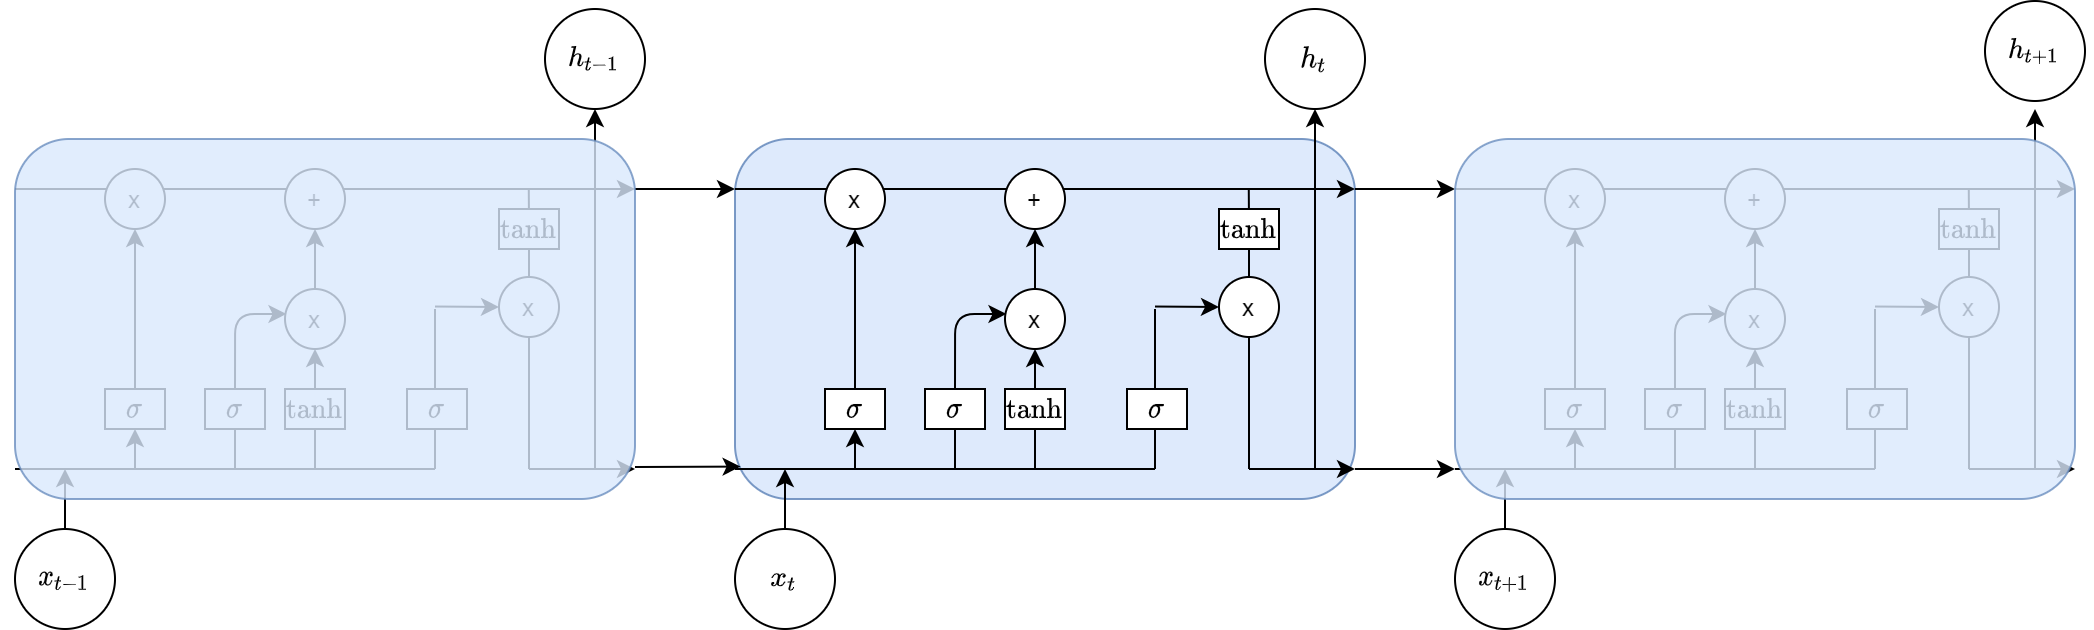
\includegraphics[scale=0.23]{02-LSTM-multiple-architecture}
\caption{Mô hình LSTM}
\end{figure}

Hình trên mô tả kiến trúc mạng LSTM. Trong đó các kí hiệu thể hiện:

	$+$ : phép cộng vector

	$\times$ : thể hiện phép nhân vector

	$tanh$ và $\sigma$ : các hàm phi tuyến
	
\begin{figure}[h]
\centering
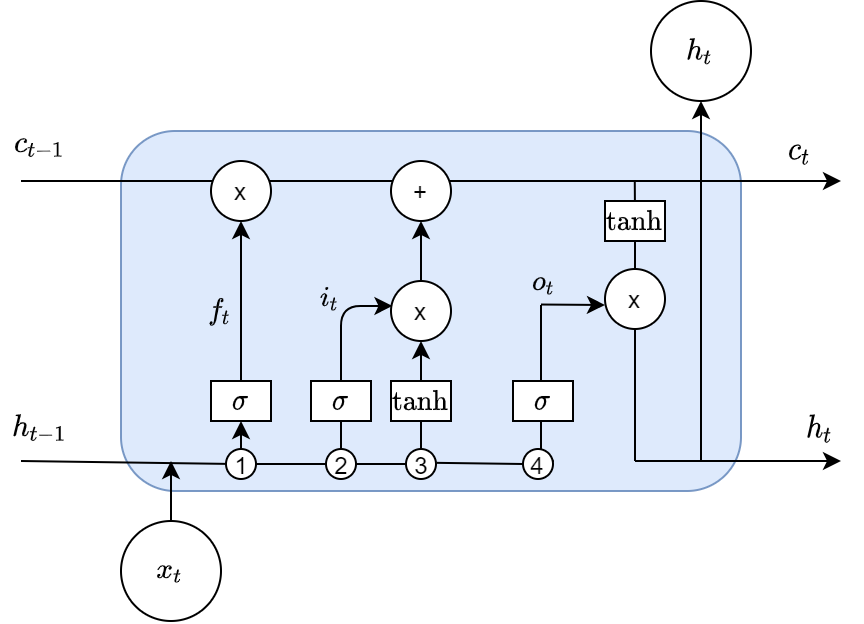
\includegraphics[scale=0.5]{02-single-LSTM}
\caption{Kiến trúc mô hình LSTM tại mỗi điểm thời gian $t$}
\end{figure}

Mô hình gồm $4$ bước: 
\textbf{\subsection{Bước $1$}
}Mạng LSTM nhìn vào các thông tin từ trạng thái $h_{t-1}$ và đầu vào $x_{t}$ để đưa ra quyết định giữ hoặc bỏ đi bằng hàm sigmoid. Đây chính là cổng giúp loại bỏ đi bớt thông tin từ trước đó.  

$f_{t} = \sigma(w_{f} \times [h_{t-1}, x_{t}] + b_{f}) \Leftarrow (1)$

\textbf{\subsection{Bước $2$}
}Bước này giúp ô trạng thái nhập nhật thông tin mới bằng biểu thức:

$i_{t} = \sigma(w_{f} \times [h_{t-1}, x_{t}] + b_{i}) \Leftarrow (2)$

$g_{t} = \tanh(w_{c} \times [h_{t-1}, x_{t}] + b_{c}) \Leftarrow (3)$

Phương trình $2$ sử dụng hàm sigmoid để quyết định thông tin nào sẽ được thêm vào ô trạng thái. 

Phương trình $3$ chuyển thông tin mới về dạng vector để có thể cộng vào ô trạng thái. 

\textbf{\subsection{Bước $3$}
}Tại bước này, ô trạng thái trước đó là $c_{t-1}$ được cập nhật vào ô trạng thái $c_{t}$ bằng cách nhân $f_{t}$ với $c_{t-1}$. Sau đó cộng với $i_{t} \times g_{t}$ để xác định nên cập nhật bao nhiêu vào trạng thái hiện tại. 

$c_{t} = f_{t} \times c_{t-1} + i_{t} \times g_{t} \Leftarrow (4)$

\textbf{\subsection{Bước 4}}
Bước này có trách nhiệm tính toán đầu ra của LSTM - vốn sẽ là đầu vào cho tầng tiếp theo trong mạng nơ-ron. Trước khi xác định đầu ra, mô hình truyền thông tin qua một hàm sigmoid để xác định thông tin gì là quan trọng. 

$o_{t} = \sigma(w_{o} \times [h_{t-1}, x_{t}] + b_{o}) \Leftarrow (5)$

$h_{t} = o_{t} \times \tanh(c_{t}) \Leftarrow (6)$

Phương trình số (6) truyền ô kết quả của trạng thái qua một hàm tanh rồi nhân kết quả với đầu ra sau khi đi qua hàm sigmoid. 

Tuy nhiên, kiến trúc LSTM trên chỉ giúp xử lý thông tin một chiều. Để cải thiện mô hình này, các đầu vào sẽ được truyền thêm vào mô hình một lần nữa nhưng theo chiều ngược lại. Kết quả từ việc truyền đầu vào theo 2 chiều rồi sẽ được ghép với nhau để biểu diễn kết quả cuối cùng. Việc kết hợp này sẽ giúp phát hiện, nắm bắt được cả sự phụ thuộc từ các từ trước hoặc sau một từ trong văn bản. Kiến trúc mạng được mô tả như dưới đây.

\begin{figure}[h]
\centering
\includegraphics[scale=0.23]{02-BiLSTM}
\caption{Kiến trúc mạng BiLSTM, các $w_{1}$, $w_{2}$, ... là các đầu vào}
\end{figure}


\end{document}